\documentclass{beamer}

\usepackage[utf8]{inputenc}
\usepackage{tikz}

\usepackage{booktabs}
\usepackage{listings}
\lstset{
  language=python,
  basicstyle=\scriptsize,
}
\usetheme{ODK}

%% \AtBeginSection[]
%% {
%%   \begin{frame}<beamer>
%%     \frametitle{Outline}
%%     \tableofcontents[currentsection]
%%   \end{frame}
%% }

\title[Workpackage 5]{Workpackage 5:\\ High Performance Mathematical Computing}

\author{Clément Pernet}

\institute[UGA]{Université Grenoble Alpes}

\begin{document}
\maketitle

%%%%%%%%%%%%%%%%%%%%%%%%%%%%%%%%%%%%%%%
\section*{Introduction}
\begin{frame}
  \frametitle{Delivering High Performance to Math VRE users}
   \begin{center}
    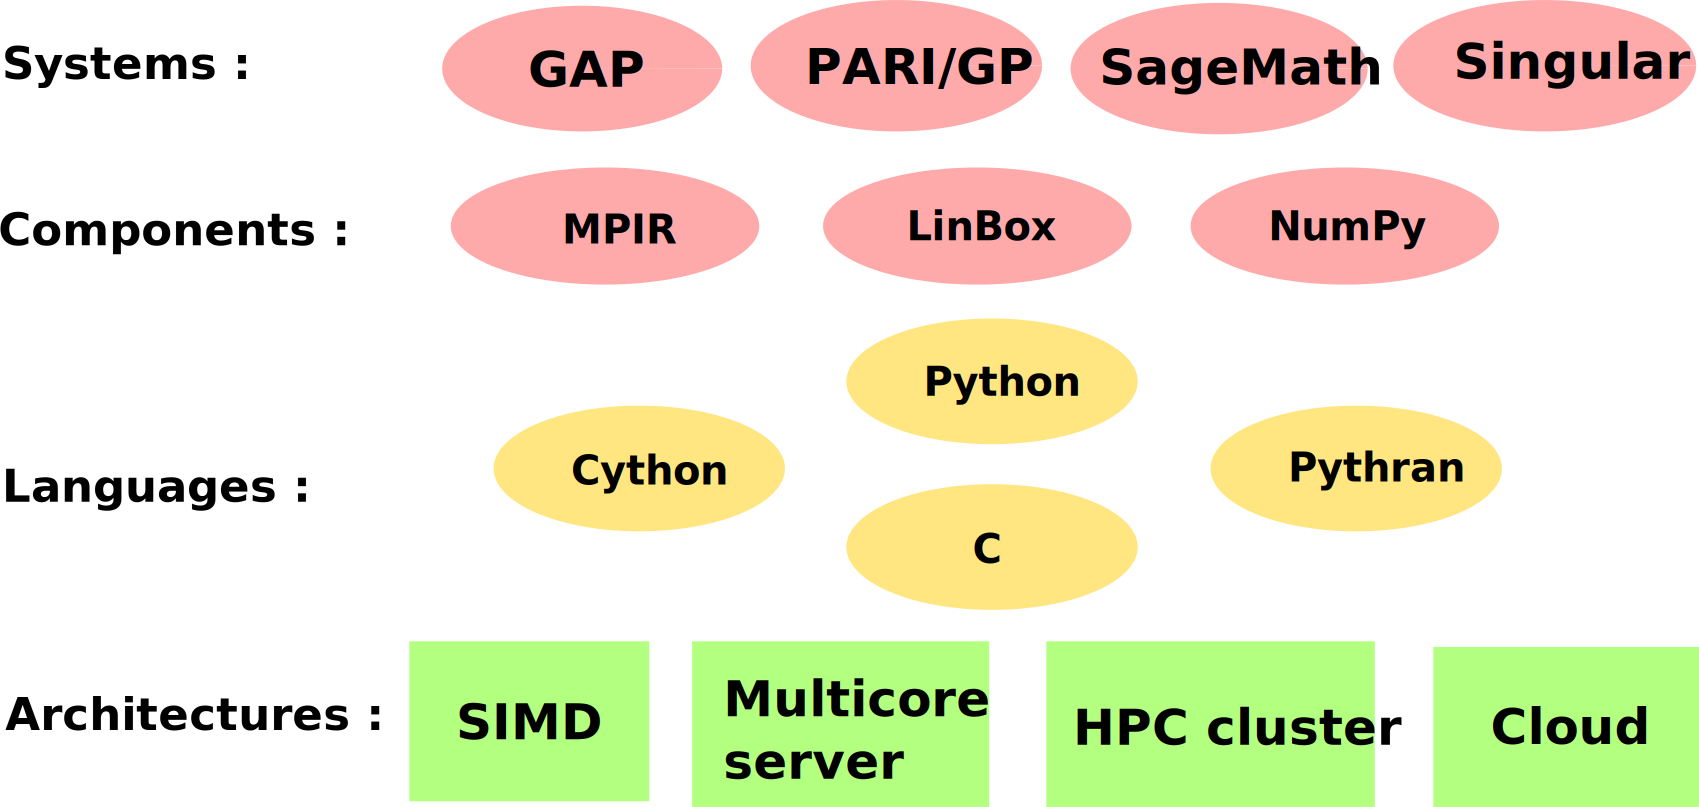
\includegraphics[width=0.8\textwidth]{software_stack}
    
  \end{center}
  
\end{frame}

%%%%%%%%%%%%%%%%%%%%%%%%%%%%%%%%%%%%%%%
\begin{frame}
  \frametitle{Introduction}
  \begin{block}
    {Goal:}
    \begin{itemize}
    \item Offer High Performance Computing to VRE's users
    \item Improve/Develop parallel computing features of dedicated software
      kernels
    \item Expose them through the software stack
    \end{itemize}
  \end{block}
\end{frame}
%%%%%%%%%%%%%%%%%%%%%%%%%%%%%%%%%%%%%%%
%%%%%%%%%%%%%%%%%%%%%%%%%%%%%%%%%%%%%%%
\section{Main tasks under review for the period}
%%%%%%%%%%%%%%%%%%%%%%%%%%%%%%%%%%%%%%%
\subsection{Task 5.4: Singular}
\begin{frame}
  \frametitle{Task 5.4: Singular}
\begin{center}{\Large
  \textbf{Singular}: a library for commutative algebra.}
\end{center}

  \begin{itemize}
  \item Already has a generic parallelization framework
  \item Focus on optimizing a few kernel routines for fine grain parallelism
  \end{itemize}

  \begin{description}
  \item[D5.6:] Quadratic sieving for integer factorization
  \item[D5.7:] Parallelization of matrix fast Fourier Transform
  \end{description}
\end{frame}
%%%%%%%%%%%%%%%%%%%%%%%%%%%%%%%%%%%%%%%
\begin{frame}
  \frametitle{D5.6: Quadratic Sieving for integer factorization}

  \begin{block}{Quadratic Sieving for integer factorization}
    \begin{description}
    \item[Problem:]  Factor an integer $n$ into prime factors
    \item[Role:] Crucial in algebraic number theory, arithmetic geometry, crypto.
    \item [Earlier status:] no HPC implementation for large instances:
      \begin{itemize}
      \item only fast code for up to 17 digits,
      \item only partial sequential implementation for large numbers
      \end{itemize}
    \end{description}
    \end{block}
\end{frame}

\begin{frame}
  \frametitle{D5.6: Quadratic Sieving for integer factorization}
    \begin{block}{Achievements}
      \begin{itemize}
      \item Completed and debugged implementation of large prime variant
      \item Parallelised sieving component of implementation using OpenMP 
      \item Experimented with a parallel implementation of Block Wiedemann
      \end{itemize}
\end{block}
\begin{block}{Results}

      \begin{itemize}
      \item Now modern, robust, parallel code for numbers in
        17--90 digit range
      \item Block Wiedemann:  \textbf{SIMD} vs \textbf{thread level}
        parallelism       \pause
%, $\leadsto$ no faster than existing code
      \item significantly faster on small multicore machines
      \end{itemize}
      \begin{center}
        \begin{table}
          \caption{Speedup for four cores (c/f single core): }
        \begin{tabular}{c|ccccc}
        \toprule
            {Digits} & 50 & 60 & 70 & 80 & 90\\
            \midrule
                {Speedup} & $1.1\times$ & $1.76\times$ & $1.55\times$ & $2.69\times$ & $2.80\times$\\
                \bottomrule
      \end{tabular}
\end{table}
      \end{center}
    \end{block}
    
\end{frame}
%%%%%%%%%%%%%%%%%%%%%%%%%%%%%%%%%%%%%%%
\begin{frame}
  \frametitle{D5.7: Parallelise and assembly optimize FFT}

  \begin{block}    {FFT: Fast Fourier Transform}
    \begin{itemize}
    \item Among the top 10 most important algorithms
    \item Key to fast arithmetic (integers, polynomials)
    \item Difficult to optimize: high memory bandwidth requirement
    \end{itemize}
    \begin{description}
    \item[Earlier status:]\
      \begin{itemize}
      \item world leading \textbf{sequential} code in MPIR and FLINT;
      \item no parallel code.
        \end{itemize}
    \end{description}
  \end{block}
\end{frame}
%%%%%%%%%%%%%%%%%%%%%%%%%%%%%%%%%%%%%%%
\begin{frame}
  \frametitle{D5.7: Parallelise and assembly optimize FFT}
  \begin{block} {Achievements}
  \begin{itemize}
\item Parallelised Matrix Fourier implementation using OpenMP 
\item Assembly optimised butterfly operations in MPIR 
\end{itemize}
  \end{block}

\begin{block}{Results:}

\begin{itemize}
\item $\approx 15\%$ speedup  on Intel Haswell
\item $\approx 20\%$ speedup on Intel Skylake  
\item Significant speedups on multicore machines
\end{itemize}
\end{block}

\vspace{-1em}
\begin{table}
  \caption{Speedup of large integer multiplication on 4/8 cores:}
  \begin{tabular}{cccccccc}
  \toprule
{Digits} & 3M & 10M & 35M & 125M & 700M & 3.3B & 14B\\
\midrule
    {4 cores} & $1.35\times$ & $2.67\times$ & $2.92\times$ & $2.92\times$ & $3.01\times$ & $2.95\times$ & $3.32\times$ \\
{8 cores} & $1.35\times$ & $3.56\times$ & $4.22\times$ & $4.36\times$ & $4.50\times$ & $4.31\times$ & $5.49\times$\\
\bottomrule
\end{tabular}
\end{table}
\end{frame}
%%%%%%%%%%%%%%%%%%%%%%%%%%%%%%%%%%%%%%%
\subsection{Task 5.5: MPIR}
\begin{frame}
  \frametitle{Task 5.5: MPIR}
\begin{center}
  {\Large  \textbf{MPIR} : a library for big integer arithmetic}
\end{center}
\begin{itemize}
  \item Bignum operations: absolutly fundamental across all of computer algebra
  \end{itemize}
  
  \begin{block}
    {D5.5: Assembly superoptimization}
    \begin{itemize}
    \item MPIR contains assembly language routines for bignum operations
    \item $\leadsto$ hand optimised for every new microprocessor
      architecture 
    \item $\leadsto \approx 3-6$ months of work for each arch.
    \item Superoptimisation: rearranges instructions to get optimal
      ordering
    \end{itemize}

    \begin{description}
      \item[Earlier status:]\
        \begin{itemize}
        \item No assembly code for recent ($> 2012$) Intel and AMD chips (Bulldozer,
          Haswell, Skylake, \dots)
        \end{itemize}
            \end{description}



    \end{block}
\end{frame}
%%%%%%%%%%%%%%%%%%%%%%%%%%%%%%%%%%%%%%%%%%%%%%%%%%%%%%%%%%%%%%%%%%%%%%%%%%%%
\begin{frame}

\frametitle{D5.5: Assembly superoptimisation}

\begin{block} {Achievements}
\begin{itemize}
\item A new assembly superoptimiser supporting recent instruction sets, including AVX 
\item Superoptimised handwritten assembly code for Haswell and Skylake 
\item Hand picked faster assembly code for Bulldozer from existing implementations 
\end{itemize}
\end{block}
\begin{block}
  {Results:}
\begin{itemize}
\item Sped up basic arithmetic operations for Bulldozer, Skylake and Haswell 
\item Noticeable speedups for bignum arithmetic for all size ranges
\end{itemize}
\end{block}

\end{frame}
%%%%%%%%%%%%%%%%%%%%%%%%%%%%%%%%%%%%%%%%%%%%%%%%%%%%%%%%%%%%%%%%%%%%%%%%%%%%%
\begin{frame}[fragile]

\frametitle{D5.5: Assembly superoptimisation}


\begin{table}
\caption{Speedups for bignum operations}
  \begin{tabular}{cccccccc}
  \toprule
{Op} & \mbox{Mul (s)} & \mbox{Mul (m)} & \mbox{Mul (b)} & \mbox{GCD (s)} & \mbox{GCD (m)} & \mbox{GCD (b)} \\
\midrule
{Haswell} & $1.18\times$ & $1.27\times$ & $1.29\times$ & $0.72\times$ & $1.45\times$ & $1.27\times$\\
{Skylake} & $1.15\times$ & $1.20\times$ & $1.22\times$ & $0.84\times$ & $1.65\times$ & $1.32\times$ \\
\bottomrule
\end{tabular}
\end{table}

s $= 512$ bits, m $= 8192$ bits, big $= 100$K bits 

No substantial speedups were found for the older, less sophisticated Bulldozer over existing assembly routines.

\end{frame}
%%%%%%%%%%%%%%%%%%%%%%%%%%%%%%%%%%%%%%%
%%%%%%%%%%%%%%%%%%%%%%%%%%%%%%%%%%%%%%%
\subsection{Task 5.6: Combinatorics}
\begin{frame}
  \frametitle{Task 5.6: Combinatorics}
\end{frame}
%%%%%%%%%%%%%%%%%%%%%%%%%%%%%%%%%%%%%%%
%%%%%%%%%%%%%%%%%%%%%%%%%%%%%%%%%%%%%%%
\subsection{Task 5.7: Pythran}
\begin{frame}
  \frametitle{Task 5.7: Pythran}
  \begin{center}
    {\Large \textbf{Pythran}: a Python to C compiler}
  \end{center}
  \begin{columns}
    \begin{column}
      {.48\textwidth }
          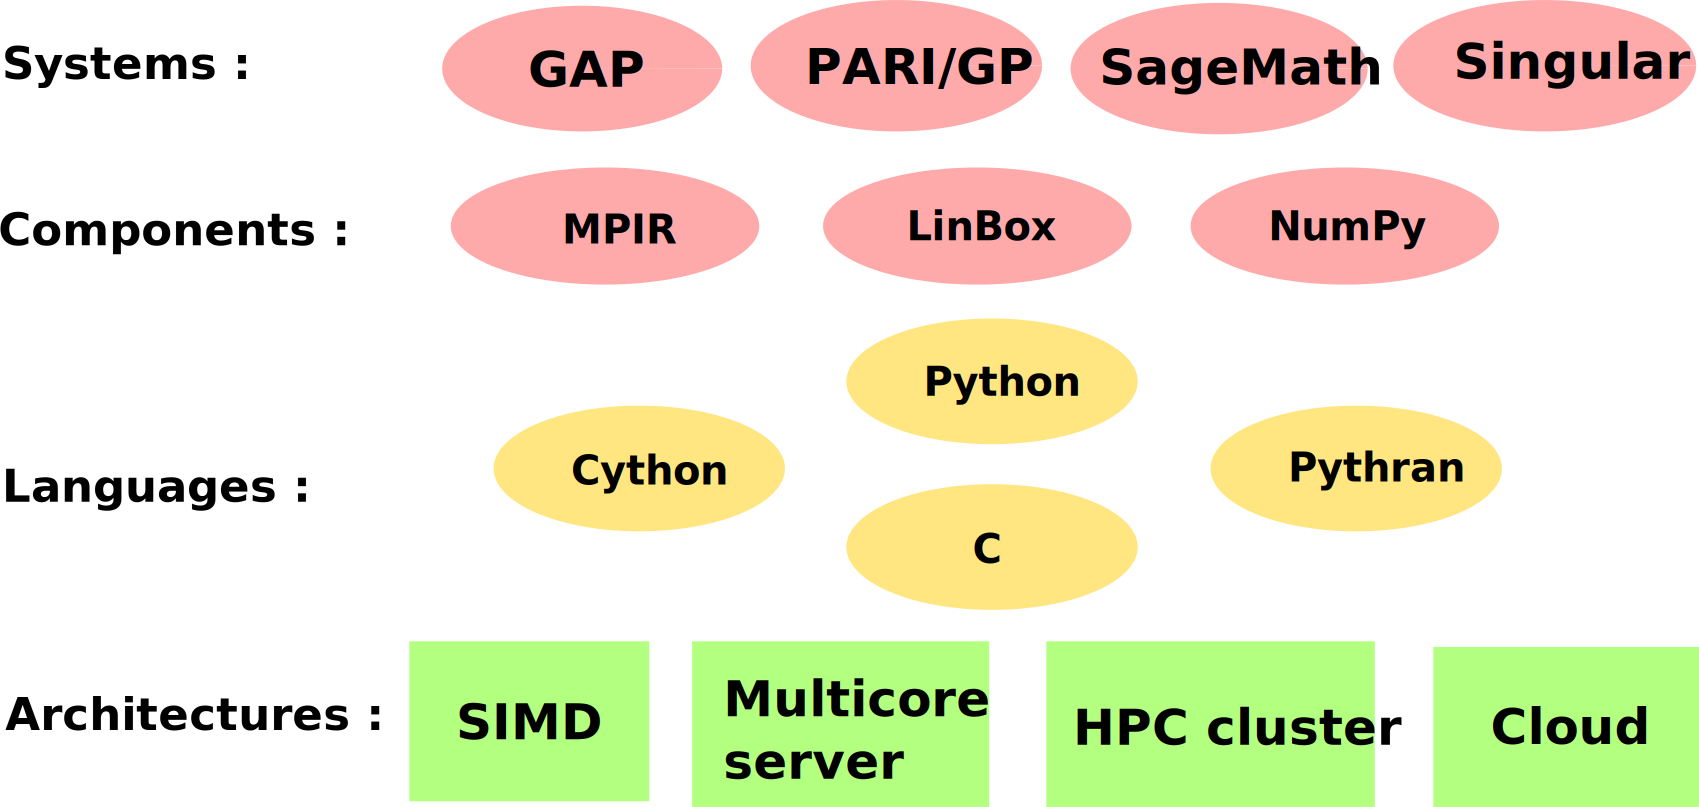
\includegraphics[width=\textwidth]{software_stack}
    \end{column}
    \begin{column}
      {.48\textwidth }
  \begin{itemize}
  \item High level VRE rely on the Python language
  \item High performance is achieved mostly by the C language\pause
  \item Python to C compilers: 
    \begin{itemize}
    \item Cython: general purpose
    \item Pythran: narrower scope, better at optimizing Numpy code (Linear
      algebra)
    \end{itemize}
  \end{itemize}
    \end{column}
  \end{columns}
\pause
  \begin{center}
    \textbf{Goal: Implement the convergence}

    \begin{description}
      \item[D5.4] Improve Pythran typing system
      \item[D5.2] Make Cython use Pythran backend to optimize Numpy code
    \end{description}
  \end{center}
  
\end{frame}
%%%%%%%%%%%%%%%%%%%%%%%%%%%%%%%%%%%%%%%
\begin{frame}[fragile]
  \frametitle{D5.2: Make Cython use Pythran backend for NumPy code}

  \begin{center}
    \includegraphics[width=.65\textwidth]{float_graph}\\
  \end{center}
  \begin{lstlisting}
import numpy
cimport numpy
def float_comp (numpy.ndarray[numpy.float_t, ndim=1] a,
                 numpy.ndarray[numpy.float_t, ndim=1] b):
     return numpy.sqrt(numpy.sqrt(a*a+b*b))
\end{lstlisting}

\end{frame}
%%%%%%%%%%%%%%%%%%%%%%%%%%%%%%%%%%%%%%%%%%%%%%%%%%%%%%%%%%%%%%%%%%
\begin{frame}[fragile]
  \frametitle{D5.2: Make Cython use Pythran backend for NumPy code}

  \begin{center}
    \includegraphics[width=.65\textwidth]{harris_graph}
  \end{center}
  
  \begin{lstlisting}[basicstyle=\tiny]
def harris(numpy.ndarray[numpy.float_t, ndim=2] I):
  cdef int m = I.shape[0]
  cdef int n = I.shape[1]
  cdef numpy.ndarray[numpy.float_t,ndim=2] dx = (I[1:,:] - I[:m-1,:])[:,1:]
  cdef numpy.ndarray[numpy.float_t,ndim=2] dy = (I[:,1:] - I[:,:n-1])[1:,:]
  cdef numpy.ndarray[numpy.float_t, ndim=2] A = dx * dx
  cdef numpy.ndarray[numpy.float_t, ndim=2] B = dy * dy
  cdef numpy.ndarray[numpy.float_t, ndim=2] C = dx * dy
  cdef numpy.ndarray[numpy.float_t, ndim=2] tr = A + B
  cdef numpy.ndarray[numpy.float_t, ndim=2] det = A * B - C * C
  return det - tr * tr
\end{lstlisting}

\end{frame}

%%%%%%%%%%%%%%%%%%%%%%%%%%%%%%%%%%%%%%%
%% \begin{frame}
%%       \frametitle{D5.4: Improve Pythran typing system}
%% \end{frame}

%%%%%%%%%%%%%%%%%%%%%%%%%%%%%%%%%%%%%%%
\subsection{Task 5.8: SunGridEngine in JupytherHub}
\begin{frame}
  \frametitle{Task 5.8: SunGridEngine integeration in JupytherHub}

  \begin{block} {Sun Grid Engine}
    A job scheduler for Academic HPC Clusters
    \begin{itemize}
    \item among the most popular
    \item 
    \end{itemize}
  \end{block}

  \begin{block}{Achievements}
  \end{block}
\end{frame}

%%%%%%%%%%%%%%%%%%%%%%%%%%%%%%%%%%%%%%%
%%%%%%%%%%%%%%%%%%%%%%%%%%%%%%%%%%%%%%%
\section{Progress report on other tasks}
\begin{frame}
  \frametitle{Progress report on other tasks}

  \begin{block}{T5.1: Pari}
    \begin{itemize}
    \item Generic parallelization engine is now mature, released (D5.10, due M24)
    \end{itemize}
  \end{block}
  \begin{block}{T5.2: GAP}
    \begin{itemize}
    \item 6 releases were cut integrating contributions of D3.11 and D5.15
    \item Build system refactoring for integration of HPC GAP
    \end{itemize}
  \end{block}
  \begin{block}{T5.3: LinBox}
    \begin{itemize}
    \item Algorithmic advances (5  articles) on linear algebra and
      verified computing
    \item Software releases and integration into SageMath
    \end{itemize}
  \end{block}
\end{frame}
%%%%%%%%%%%%%%%%%%%%%%%%%%%%%%%%%%%%%%%
%% \subsection{Task 5.1: Pari}
%% \begin{frame}
%%   \frametitle{Task 5.1: Pari}
%% \end{frame}
%% %%%%%%%%%%%%%%%%%%%%%%%%%%%%%%%%%%%%%%%
%% \subsection{Task 5.2: GAP}
%% \begin{frame}
%%   \frametitle{Task 5.1: GAP}
%% \end{frame}
%% %%%%%%%%%%%%%%%%%%%%%%%%%%%%%%%%%%%%%%%
%% \subsection{Task 5.3: LinBox}
%% \begin{frame}
%%   \frametitle{Task 5.3: LinBox}
%% \end{frame}
%%%%%%%%%%%%%%%%%%%%%%%%%%%%%%%%%%%%%%%
%%%%%%%%%%%%%%%%%%%%%%%%%%%%%%%%%%%%%%%
\end{document}
